\documentclass[final]{beamer}

% Declare the poster size to beamerposter UP FRONT (36in x 48in = 91.44 x 121.92 cm).
% Do NOT reset \paperwidth/\paperheight afterwards: that desyncs the text area.
\usepackage[orientation=portrait, size=custom, width=91.44, height=121.92,
  scale=1.3]{beamerposter}
\usetheme{confposter}

% Make the text area span the full paper width so column widths are predictable
\setbeamersize{text margin left=0pt, text margin right=0pt}

\usepackage{graphicx}
\usepackage{booktabs}

%-----------------------------------------------------------
% Neutral slate palette
%-----------------------------------------------------------
\definecolor{slate}{HTML}{3F4E5A}
\definecolor{ink}{HTML}{22303C}
\definecolor{bordergray}{HTML}{CBD2D8}

\setbeamercolor{block title}{fg=slate,bg=white}
\setbeamercolor{block body}{fg=ink,bg=white}
\setbeamercolor{block alerted title}{fg=white,bg=slate}
\setbeamercolor{block alerted body}{fg=ink,bg=slate!8}
\setbeamercolor{item}{fg=slate}
\setbeamercolor{item projected}{fg=white,bg=slate}
\setbeamercolor{structure}{fg=slate}

%-----------------------------------------------------------
% Two-column geometry (fractions of \paperwidth, summed < 1 for slack)
% 0.025 + 0.46 + 0.025 + 0.46 + 0.025 = 0.995
%-----------------------------------------------------------
\newlength{\sepwid}
\newlength{\onecolwid}
\setlength{\sepwid}{0.025\paperwidth}
\setlength{\onecolwid}{0.46\paperwidth}

%-----------------------------------------------------------
% Reusable lorem paragraph
%-----------------------------------------------------------
\newcommand{\lp}{Lorem ipsum dolor \textbf{sit amet}, consectetur adipiscing
  elit. Sed commodo molestie porta. Sed ultrices scelerisque sapien ac
  commodo. Donec ut volutpat elit. Sed laoreet accumsan mattis. Integer sapien
  tellus, auctor ac blandit eget, sollicitudin vitae lorem. Praesent dictum
  tempor pulvinar. Suspendisse potenti. Sed tincidunt varius ipsum, et porta
  nulla suscipit et. Etiam congue bibendum felis, ac dictum augue cursus a.}

%-----------------------------------------------------------
% Header: logo (left) + title (centre), full-width rule, author band
%-----------------------------------------------------------
\newcommand{\logoplaceholder}{%

\includegraphics[width=10cm]{media/tcs_research_logo.jpeg}
  
  }

\setbeamertemplate{headline}{
  \leavevmode
  \vskip1.5cm
  \begin{columns}[c]
    \begin{column}{0.02\paperwidth}\end{column}
    \begin{column}{0.20\paperwidth}
      \centering \logoplaceholder
    \end{column}
    \begin{column}{0.54\paperwidth}
      \centering
      {\color{slate}\bfseries\Huge \inserttitle}
    \end{column}
    \begin{column}{0.20\paperwidth}\end{column}
    \begin{column}{0.02\paperwidth}\end{column}
  \end{columns}
  \vskip1.0cm
  \begin{center}
    {\color{slate}\Large \insertauthor\par}\vskip0.35cm
    {\color{slate}\large \insertinstitute\par}
  \end{center}
  \vskip1.0cm
  \begin{center}{\color{bordergray}\rule{0.95\paperwidth}{3pt}}\end{center}
  \vskip1.0cm
}

%-----------------------------------------------------------
% Image placeholder: #1 = height (e.g. 18cm), #2 = caption
% Replace the tikzpicture with 
%-----------------------------------------------------------
\newcommand{\gymImg}[2]{%
  % \begin{center}
  %   \begin{tikzpicture}
  %     \node[draw=bordergray, line width=2pt, fill=slate!5,
  %           minimum width=0.9\linewidth, minimum height=#1,
  %           align=center, text=slate, font=\Large]{Placeholder Image};
  %   \end{tikzpicture}\\[0.4cm]
  %   {\small\itshape #2}
  % \end{center}
  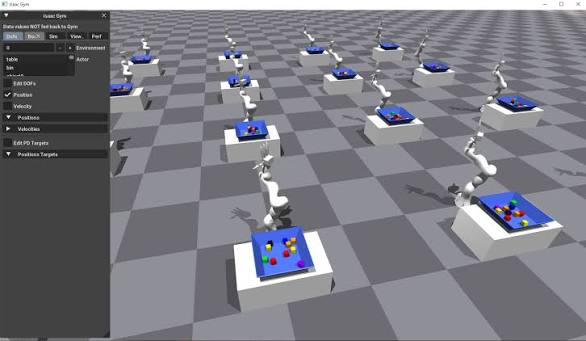
\includegraphics[width=0.9\linewidth]{media/gym.jpeg}
  }



\newcommand{\imgph}[2]{%
  % \begin{center}
  %   \begin{tikzpicture}
  %     \node[draw=bordergray, line width=2pt, fill=slate!5,
  %           minimum width=0.9\linewidth, minimum height=#1,
  %           align=center, text=slate, font=\Large]{Placeholder Image};
  %   \end{tikzpicture}\\[0.4cm]
  %   {\small\itshape #2}
  % \end{center}
  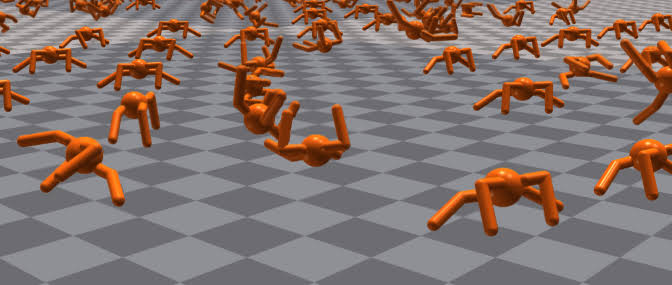
\includegraphics[width=0.9\linewidth]{media/ant.jpeg}
  }

%-----------------------------------------------------------
% Title metadata
%-----------------------------------------------------------
\title{Poster Title Goes Here}
\author{First Author, Second Author, and Third Author}
\institute{Department, University Name}

\begin{document}

\addtobeamertemplate{block end}{}{\vspace*{2ex}}
\addtobeamertemplate{block alerted end}{}{\vspace*{2ex}}
\setlength{\belowcaptionskip}{2ex}
\setlength\belowdisplayshortskip{2ex}

\begin{frame}[t]
\begin{columns}[t]

  \begin{column}{\sepwid}\end{column}

  % ===================== LEFT COLUMN =====================
  \begin{column}{\onecolwid}

    \begin{alertblock}{Objectives}
      \lp
      \begin{itemize}
        \item First objective, stated concisely.
        \item Second objective with a measurable outcome.
        \item Third objective or hypothesis under test.
        \item Fourth objective for completeness.
      \end{itemize}
    \end{alertblock}

    \begin{block}{Introduction}
      \lp

      \lp
      \gymImg{16cm}{Figure 1: Figure caption.}
    \end{block}

    \begin{block}{Materials}
      The following materials were required to complete the research:
      \begin{itemize}
        \item Curabitur pellentesque dignissim
        \item Eu facilisis est tempus quis
        \item Duis porta consequat lorem
      \end{itemize}
      They were prepared according to the steps below:
      \begin{enumerate}
        \item Curabitur pellentesque dignissim
        \item Eu facilisis est tempus quis
        \item Duis porta consequat lorem
      \end{enumerate}
    \end{block}

    \begin{block}{Methods}
      \lp
      \begin{equation}
        E = mc^{2}
      \end{equation}
      \lp
      \begin{equation}
        \kappa = \frac{\xi}{E_{\mathrm{max}}}
      \end{equation}
    \end{block}

  \end{column}

  \begin{column}{\sepwid}\end{column}















  % ===================== RIGHT COLUMN =====================
  \begin{column}{\onecolwid}

    \begin{block}{Results}
      \imgph{18cm}{Figure 2: Figure caption.}

      \lp

      \begin{table}
        \vspace{2ex}
        \begin{tabular}{l l l}
          \toprule
          \textbf{Treatments} & \textbf{Res. 1} & \textbf{Res. 2}\\
          \midrule
          Treatment 1 & 0.0003262 & 0.562 \\
          Treatment 2 & 0.0015681 & 0.910 \\
          Treatment 3 & 0.0009271 & 0.296 \\
          \bottomrule
        \end{tabular}
        \caption{Table caption.}
      \end{table}

      \lp
    \end{block}

    \begin{block}{Discussion}
      \lp

      \lp
    \end{block}

    \begin{block}{Conclusion}
      \lp
    \end{block}

    \begin{block}{References}
      \small
      \begin{thebibliography}{9}
        \bibitem{ref1} A. Author, B. Author. \textit{Title of the referenced
          work}. Publisher, 2024.
        \bibitem{ref2} C. Author, D. Author. \textit{Title of a journal
          article}. Journal Name, 12(3):45--67, 2025.
      \end{thebibliography}
    \end{block}

    \begin{alertblock}{Contact}
      \begin{itemize}
        \item Web: \texttt{https://www.example.edu/lab}
        \item Email: \texttt{name@example.edu}
        \item Phone: +91 000 000 0000
      \end{itemize}
    \end{alertblock}

  \end{column}

  \begin{column}{\sepwid}\end{column}

\end{columns}
\end{frame}

\end{document}